% Full body and appendix for convenient reading. Compile paper.tex in the complete ZIP project.

\section{Introduction}
\label{sec:introduction}

A medical model may be asked to describe an image, explain a diagnosis, or choose among a small set of alternatives. These requests share an input interface, but they do not require the same output computation. Report writing requires language generation. Selecting an answer to a multiple-choice question requires a decision. When the alternatives are already given, generating a string is one way to communicate that decision, rather than a requirement of the task itself.

This distinction has become timely with TypeSafe's release of Jev on September 15, 2026~\cite{jev}. Jev presents a System One interface that returns structured probabilistic decisions instead of free-form text. The release brings renewed attention to a longstanding question in a new deployment setting: how much of a generative model is needed when software consumes a bounded answer? Direct classification and discriminative medical VQA predate this release~\cite{q2a,kasa}. What has changed is the opportunity to examine these choices using strong pretrained medical models and an emerging family of decision-oriented systems.

The opportunity is especially relevant to multimodal medicine. A model must combine the question and candidate meanings with visual evidence, while allocating computation between image processing, representation learning, and output production. Removing answer decoding may save time without changing the representation. Learning a decision head may improve discrimination while adding supervision and candidate-scoring cost. Replacing the backbone may reduce computation further but change the knowledge and visual information available to the decision. These interventions should therefore be evaluated separately before being grouped under a single System One label.

\begin{figure}[t]
\centering
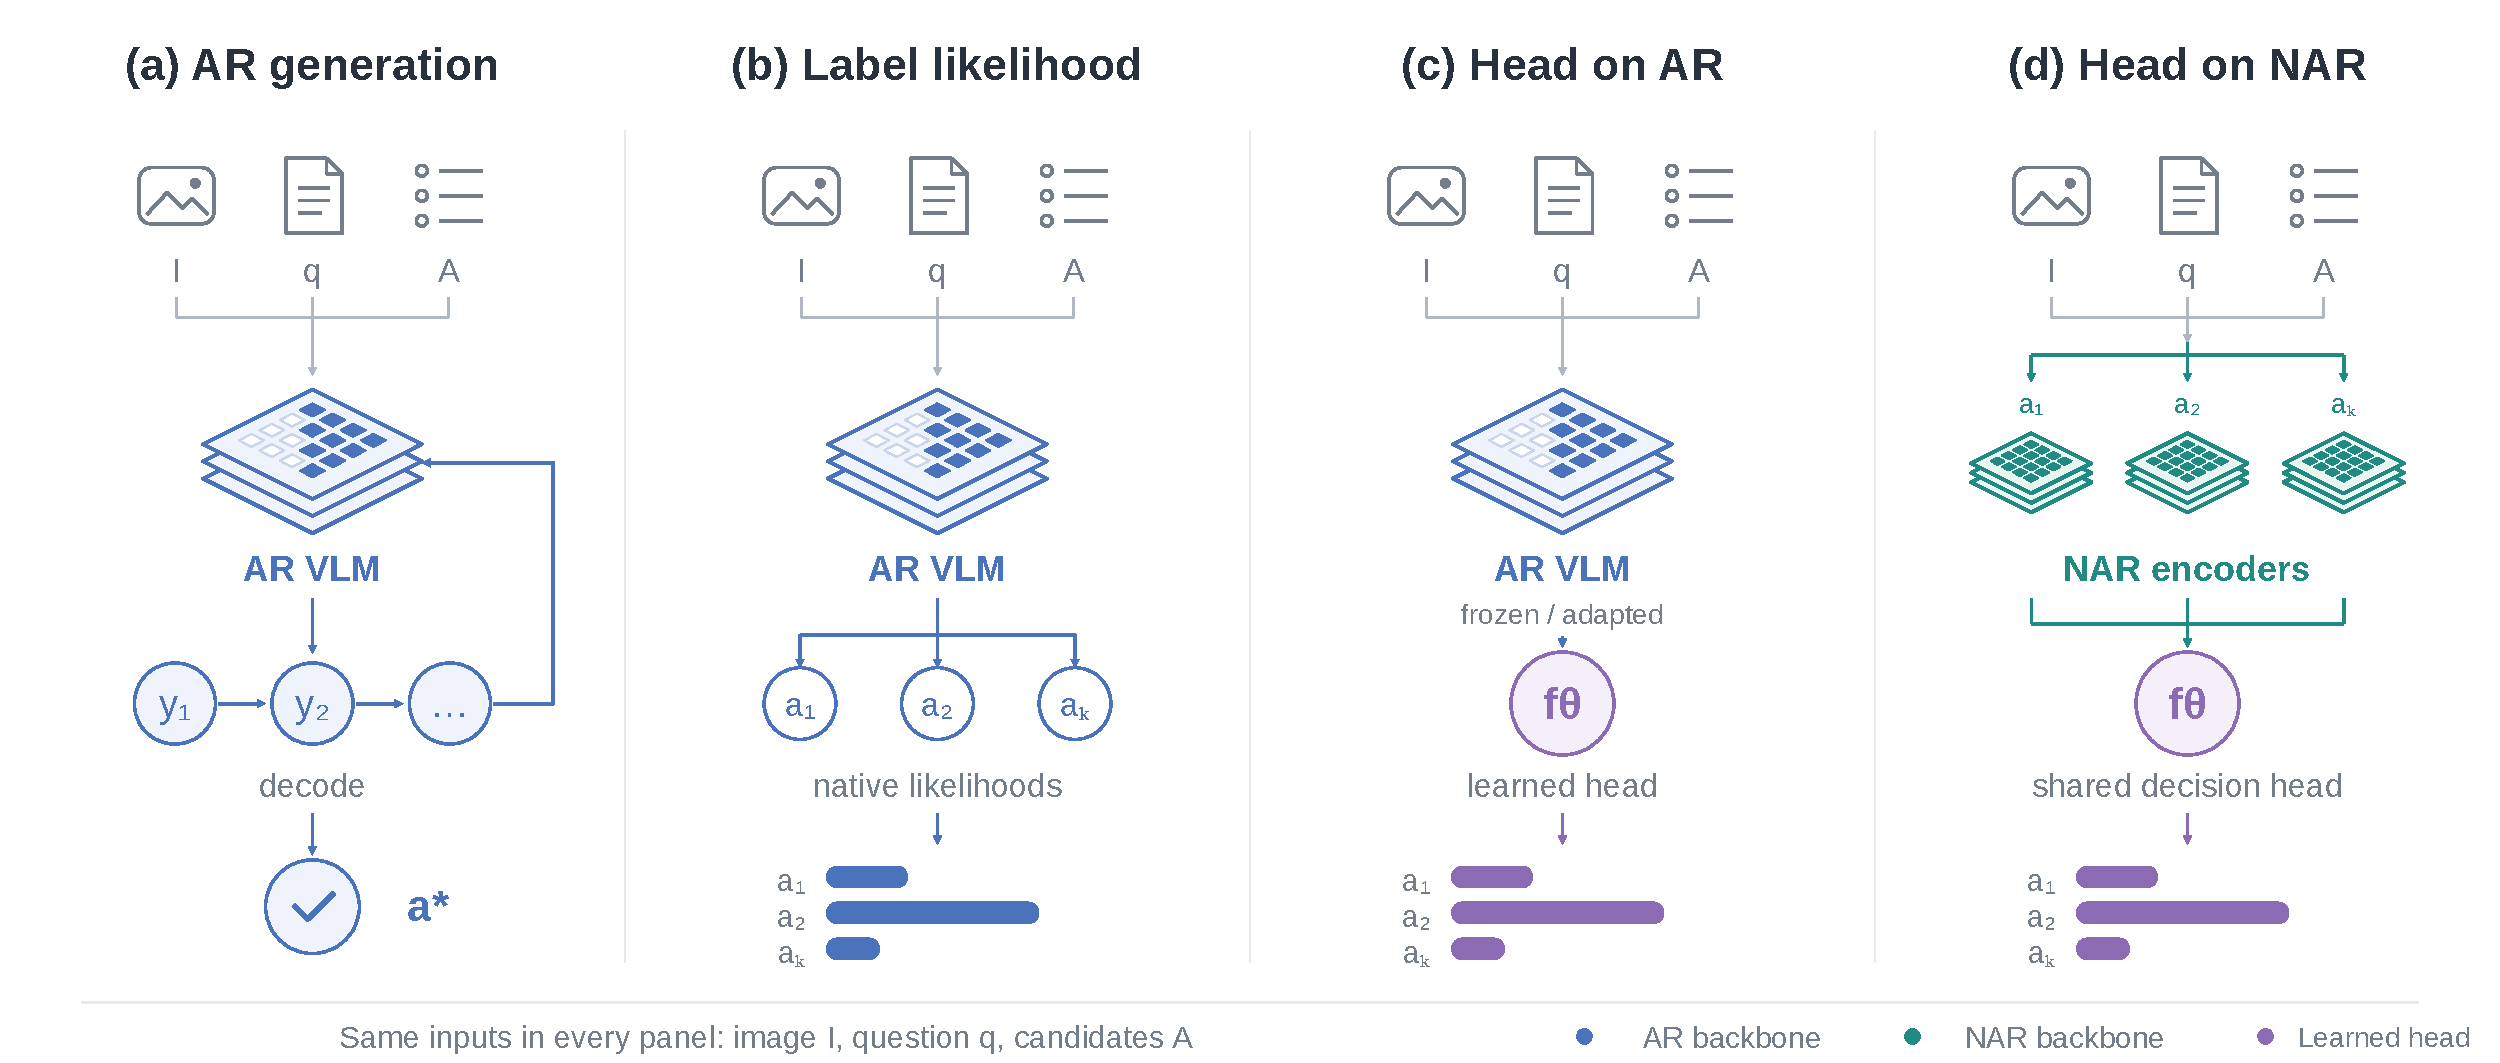
\includegraphics[width=\linewidth]{assets/figures/decision_formulations_refined.pdf}
\caption{\textbf{The design space studied by Medical SysOne.} Each formulation receives an image when available, a question, and an allowed candidate set. Moving from (a) to (b) changes the output interface; (c) adds supervised decision learning, with frozen or adapted backbone weights; (d) changes the representation family as well. The panels organize comparisons, not a sequence of guaranteed improvements. Cross-family differences cannot be attributed to attention direction alone.}
\label{fig:formulations}
\end{figure}

We address this problem through \sysone, an empirical study of bounded medical decisions. Figure~\ref{fig:formulations} distinguishes four formulations: autoregressive answer generation, native candidate-label likelihood scoring, learned heads on autoregressive backbones, and learned heads on non-autoregressive encoders. MedGemma provides the backbone for the first three formulations. MedGemma-Head and MedGemma-LoRA separate frozen-representation decision learning from parameter-efficient backbone adaptation. Laya-Med extends the comparison to a biomedical encoder-based multimodal configuration. Jev, MedJev, and Laya provide context from existing decision systems, with their modality restrictions made explicit.

Our central question is not whether generation can be removed---a classifier already establishes that possibility---but \emph{what is retained, gained, or lost when different parts of a pretrained medical decision pipeline are changed}. We examine accuracy, probability quality, and recorded inference cost, then consider policies that decide whether a fixed model should answer or defer. The distinction between a model and its decision policy is essential: higher accuracy among retained answers is not the same as a better predictor on all examples.

The available results reveal a non-monotonic design space. MedGemma likelihood scoring matches the reported accuracy of generation on every dataset, but learned heads improve visual accuracy at a higher recorded cost than likelihood readout. Laya-Med performs strongly on several visual benchmarks while falling behind on PMC-VQA and text tasks. These reversals motivate task-specific design choices rather than a universal architecture ranking. We organize the study around four questions: \textbf{RQ1}, what changes when answer decoding is removed; \textbf{RQ2}, what supervised heads and backbone adaptation add; \textbf{RQ3}, where encoder-based multimodal decisions remain competitive; and \textbf{RQ4}, what fixed-model confidence can support at inference time.

Our contribution has three parts. First, we provide a formulation-based comparison that distinguishes decoding, learned readout, backbone adaptation, and representation family. Second, we use multimodal medical configurations to expose trade-offs that text-only decision models cannot resolve. Third, we separate predictive quality from decision-policy evaluation, including the assumptions needed to interpret calibration, selection, and conformal sets. The resulting study is intended to guide the construction and evaluation of bounded medical decision models, without presenting the configurations as a new foundation model.

\authorcheck{This manuscript reproduces the baseline values in the supplied draft. The current evidence is preliminary: sample identities, training settings, and timing boundaries require confirmation. Conflicting post-hoc exports are documented in Appendix~\ref{app:audit} and are not used to claim a verified reliability improvement.}

\section{Related Work}
\label{sec:related}

\textbf{Generation and direct prediction.} The generative--discriminative distinction has long shaped classification. Recent transformer comparisons examine not only accuracy but also calibration, data efficiency, and practical constraints~\cite{kasa}. In vision--language modeling, candidate text can also be scored through a generative model's likelihoods, although such scores may depend strongly on language priors~\cite{visualgpt}. These results establish that generation-trained representations and a generative output interface are separate choices. Our study applies this distinction to bounded medical QA and VQA, where both the source of evidence and the decision interface can affect the outcome.

\textbf{Medical multimodal decisions.} Medical VQA includes classification, generation, and hybrid approaches. Q2ATransformer uses candidate-answer embeddings to query fused image--question features~\cite{q2a}, while PMC-VQA studies medical visual instruction tuning through a generative formulation~\cite{pmcvqa}. A recent comparative study also evaluates classification-style and generative VLMs with fine-tuning and post-hoc answer selection~\cite{systematicvqa}. Thus, direct medical answer selection is established prior art. MedGemma supplies a more recent medical vision--language backbone for examining native likelihoods and learned heads within one model family~\cite{medgemma}. Our focus is the relationship between those interfaces, their supervision, and their accuracy--cost trade-offs.

\textbf{System One decision interfaces.} Jev exposes typed probabilistic outputs~\cite{jev}. Jevify-style implementations adapt existing language models to comparable interfaces~\cite{jevify}, Kev learns decisions over causal language-model representations~\cite{kev}, and MedJev applies this direction to clinical variable extraction from text~\cite{medjev}. Laya instead uses non-autoregressive encoders for text-based decisions~\cite{laya}. We use these systems to locate practical design points, not as evidence that the underlying techniques are newly invented. Jev's internal architecture remains undisclosed, so it is not assigned to an AR or NAR backbone category.

\textbf{Confidence and abstention.} Temperature scaling studies the relationship between scores and empirical correctness~\cite{guo}. Selective prediction evaluates the trade-off between answering more examples and making fewer errors on accepted examples~\cite{selective,reliablevqa}. Conformal prediction provides prediction-set coverage under specified assumptions~\cite{conformal}; MedAbstain studies abstention in medical multiple-choice QA~\cite{medabstain}. JEV-as-a-Judge further examines confidence-based escalation to a stronger judge~\cite{jevjudge}. These policies are established tools. The question here is how their usefulness depends on the decision distribution produced by each modeling choice.

\section{Study Design}
\label{sec:design}

\subsection{Bounded decisions and four formulations}

Let $x=(c,q,I)$ contain a text context $c$, question $q$, and optional image $I$. Each example also supplies an ordered set of candidate answers $A=\{a_1,\ldots,a_K\}$ and a target index $y\in\{1,\ldots,K\}$. A direct decision model returns $p(y=j\mid x,A)$ and predicts $\hat y=\arg\max_j p_j$. The candidate set may vary between examples; a candidate-conditioned scorer is therefore distinct from a classifier tied to one global answer vocabulary. Our scope is selection within the supplied alternatives. It does not establish that the alternatives are exhaustive or that the selected answer is clinically correct outside the benchmark.

\textbf{AR generation.} A vision--language model receives the evidence and alternatives, then emits a token sequence $s$ with
\begin{equation}
 p_{\phi}(s\mid x,A)=\prod_{t=1}^{|s|}p_{\phi}(s_t\mid x,A,s_{<t}).
\end{equation}
A parser maps the sequence to an allowed answer. Output length, stopping criteria, and invalid-answer handling are part of this pipeline. An efficient constrained one-token decoder is a relevant control because its cost can be close to that of reading next-token candidate probabilities.

\textbf{Candidate-label likelihood scoring.} The same AR backbone can expose scores over answer identifiers without producing an answer sequence. If $\mathcal V_j$ contains the token forms assigned to candidate $j$, a label-mass readout has the form
\begin{equation}
 u_j=\sum_{v\in\mathcal V_j}p_\phi(v\mid x,A),\qquad
 p_j^{\mathrm{LL}}=\frac{u_j}{\sum_{\ell=1}^{K}u_\ell}.
\label{eq:ll}
\end{equation}
This describes candidate-label scoring, not full candidate-answer sequence likelihood. The token mapping, any top-$k$ truncation, and missing-mass handling must be specified for reproducibility. Removing the output loop leaves prompt and image processing intact; its benefit therefore depends on the workload.

\textbf{Learned heads on AR representations.} A learned scorer maps backbone representations to candidate logits, $z_j=f_\theta(h_\phi(x,A),a_j)$, followed by normalization across candidates. This notation accommodates different pooling and candidate representations without assuming a particular implementation. MedGemma-Head learns the decision interface while keeping the pretrained backbone fixed. MedGemma-LoRA additionally adapts the backbone using low-rank updates~\cite{lora}. Their comparison asks whether task supervision is better absorbed by the readout alone or also by the underlying representation. Comparing either with native likelihoods changes supervision as well as the interface; it is not a training-free replacement.

\textbf{Learned heads on NAR representations.} Laya-Med uses biomedical text and image encoders in place of an autoregressive VLM. The supplied architecture combines candidate-conditioned PubMedBERT representations~\cite{pubmedbert} with a shared BiomedCLIP image representation~\cite{biomedclip}. Abstractly,
\begin{equation}
 t_j=E_{\mathrm{text}}(c,q,A,a_j),\quad
 v=E_{\mathrm{image}}(I),\quad
 z_j=f_\theta([P_t t_j;P_v v]).
\label{eq:laya}
\end{equation}
The image embedding is reused across candidates, and the scoring head shares parameters across alternatives. For text-only tasks the visual branch is absent; the exact missing-image representation is an implementation detail to record. The architecture diagram specifies LoRA in the encoders and trainable projections and head. It describes a practical multimodal decision configuration, rather than an isolated intervention on attention direction.

\begin{table}[t]
\centering\small
\setlength{\tabcolsep}{4pt}\renewcommand{\arraystretch}{1.15}
\caption{\textbf{Formulations and comparison roles.} AR/NAR describes the backbone family; decoding describes the output process. All three constructed configurations use text and images. External systems supply context but do not isolate an architectural factor.}
\label{tab:taxonomy}
\begin{tabularx}{\linewidth}{@{}l l X l@{}}
\toprule
\textbf{Configuration} & \textbf{Input} & \textbf{Decision mechanism} & \textbf{Backbone update}\\
\midrule
MedGemma-AR & Text + image & AR answer generation & None\\
MedGemma-LL & Text + image & Native label-likelihood readout & None\\
MedGemma-Head & Text + image & Learned decision head on AR VLM & Frozen\\
MedGemma-LoRA & Text + image & Learned decision head on AR VLM & LoRA\\
Laya-Med & Text + image & Shared head on biomedical encoders & LoRA\\
\midrule
Jev & Text/structured & Proprietary direct decisions & Undisclosed\\
MedJev & Text & Learned decisions on causal LM & LoRA\\
Laya & Text & NAR decision engine & Model-specific\\
\bottomrule
\end{tabularx}
\end{table}


\subsection{What each comparison identifies}

Table~\ref{tab:taxonomy} separates the locally constructed configurations from external systems. The strongest within-family contrast is MedGemma generation versus MedGemma likelihood scoring, provided both use the same checkpoint and input preparation. Frozen-head versus adapted-head comparison then tests the incremental effect of backbone adaptation under matched training. In contrast, native readout versus a trained head includes additional labeled supervision. A matched adapted-backbone likelihood baseline is needed to isolate the benefit of the head after adaptation.

The transition to Laya-Med changes pretraining, model size, image encoding, fusion, and training in addition to the backbone family. We therefore interpret RQ3 as a comparison of available configurations. Likewise, Jev, MedJev, and Laya are contextual baselines: differences in their training objectives and supported tasks constrain the conclusions that can be drawn from their scores. MedJev's clinical extraction objective, for example, differs from medical examination QA~\cite{medjev}.

\subsection{Benchmarks and evaluation quantities}

The study spans PubMedQA, MedQA, and MedMCQA for text-based questions, and VQA-RAD, SLAKE, PathVQA, and PMC-VQA for visual questions~\cite{pubmedqa,medqa,medmcqa,vqarad,slake,pathvqa,pmcvqa}. These datasets sample different sources of medical evidence. Their names alone do not specify the evaluated task: visual QA collections contain different answer types, and a bounded evaluation may use closed-ended subsets or a constructed candidate set. Appendix~\ref{app:protocol} lists the exact protocol fields that remain to be confirmed for the current result export. We do not equate the reported subset results with official full-benchmark performance.

\textbf{Accuracy and aggregation.} Accuracy is the proportion of examples assigned the correct candidate. We report each dataset separately and macro-average only over a common task set: three text datasets or four visual datasets. Text-only systems are excluded from visual averages. We omit an overall ranking that would compare a three-task average for one system with a seven-task average for another. Equal dataset-level accuracy does not establish identical example-level predictions.

\textbf{Probability quality.} For models with distributions over the same candidate support, negative log-likelihood is $\mathrm{NLL}=-N^{-1}\sum_i\log p_{i,y_i}$. The multiclass Brier score is $N^{-1}\sum_i\sum_j(p_{i,j}-\mathbf 1[y_i=j])^2$. Expected calibration error compares mean confidence with empirical accuracy within confidence bins. NLL and Brier assess the full probability distribution; ECE depends on the confidence definition and binning. A free-form answer's token likelihood is not automatically comparable to a normalized candidate probability. The draft's calibration plot is therefore not sufficient to establish a common probability protocol across all rows.

\textbf{Inference cost.} We reproduce the recorded dataset-level median latency in milliseconds. A mean of dataset medians is labeled as such and is not a pooled request median. Local forward time, amortized batch time, and hosted-service wall time measure different costs. Until batch size, precision, preprocessing, caching, and synchronization are aligned, these values describe the recorded implementations rather than a hardware-controlled architectural speedup. Throughput and memory are not inferred from the supplied medians.

\textbf{Evidence scope.} The post-hoc table explicitly reports 50 examples per dataset. Corresponding sample counts and IDs for every baseline row need confirmation, and per-example predictions are not part of the supplied draft. We report descriptive differences without significance tests, confidence intervals, or claims of repeated-seed robustness. This scope matters particularly when a difference of a few percentage points may correspond to only a small number of decisions.

\section{What Determines Decision Quality and Cost?}
\label{sec:results}

Table~\ref{tab:accuracy} presents the baseline accuracy values from the supplied draft. Table~\ref{tab:latency} separates the corresponding recorded latencies, so that predictive behavior and implementation cost can be examined without compressing both into one color scale. Figures~\ref{fig:tradeoff} and~\ref{fig:contrasts} summarize the resulting patterns. All arithmetic in this section is derived from those reported values; no new model evaluation is implied.

\begin{table}[t]
\centering\scriptsize\setlength{\tabcolsep}{3.4pt}\renewcommand{\arraystretch}{1.23}
\caption{\textbf{Reported baseline accuracy on seven medical decision tasks.} Values reproduce the supplied landscape table. Text and visual means use three and four common datasets, respectively; unsupported tasks are marked --. These are descriptive export values, not newly run experiments or claims of official full-test performance.}
\label{tab:accuracy}
\begin{tabular*}{\linewidth}{@{\extracolsep{\fill}}lrrrrrrrrr@{}}
\toprule
 & \multicolumn{3}{c}{\textbf{Text tasks}} & \multicolumn{4}{c}{\textbf{Visual tasks}} & \multicolumn{2}{c}{\textbf{Task means}}\\
\cmidrule(lr){2-4}\cmidrule(lr){5-8}\cmidrule(lr){9-10}
\textbf{Method} & PubMed & MedQA & MedMC & RAD & SLAKE & Path & PMC & Text & Visual\\
\midrule
MedGemma-AR & 66.0 & 48.0 & 66.0 & 78.0 & 74.0 & 70.0 & 48.0 & 60.0 & 67.5\\
MedGemma-LL & 66.0 & 48.0 & 66.0 & 78.0 & 74.0 & 70.0 & 48.0 & 60.0 & 67.5\\
Jev & 88.0 & 96.0 & 80.0 & -- & -- & -- & -- & 88.0 & --\\
MedJev & 56.0 & 24.0 & 38.0 & -- & -- & -- & -- & 39.3 & --\\
Laya & 54.0 & 22.0 & 20.0 & -- & -- & -- & -- & 32.0 & --\\
\midrule
\textcolor{PaperPurple}{MedGemma-Head} & 62.0 & 52.0 & 70.0 & 82.0 & 88.0 & 96.0 & 52.0 & 61.3 & 79.5\\
\textcolor{PaperPurple}{MedGemma-LoRA} & 72.0 & 52.0 & 66.0 & 82.0 & 84.0 & 96.0 & 68.0 & 63.3 & 82.5\\
\textcolor{PaperTeal}{Laya-Med} & 66.0 & 26.0 & 44.0 & 94.0 & 90.0 & 94.0 & 34.0 & 45.3 & 78.0\\
\bottomrule
\end{tabular*}
\end{table}


\subsection{RQ1: What changes when answer decoding is removed?}

MedGemma generation and candidate-label likelihood scoring have the same reported accuracy on all seven datasets. Both average 60.0\% on text tasks and 67.5\% on visual tasks. The result supports a narrow but useful observation: in this evaluation, the sequence-generation interface contributes no observed dataset-level accuracy advantage over direct label readout. It does not show that the predictions are identical or that generation is unnecessary for all medical questions.

The recorded cost changes substantially. Text-task medians fall from 1,087--1,141\,ms for generation to 38--55\,ms for likelihood scoring; visual-task medians fall from 1,230--1,337\,ms to 158--168\,ms. The reported within-dataset ratios range from 7.5 to 29.6. These are ratios of the supplied timing measurements, conditional on their measurement boundaries. The smaller visual-task reduction is consistent with input processing occupying a larger fraction of inference, although timing decomposition is needed to test that explanation.

\finding{Finding 1.}{The reported accuracy is unchanged when MedGemma's output interface changes from generation to label scoring, while its recorded inference cost decreases. This establishes the value of the comparison, not a universal advantage over an optimized one-token decoder.}

This distinction changes the next question. Once the output loop has been removed, any further predictive gain must come from the information used by the decision or the way that information is learned and read out. RQ2 examines these changes within the MedGemma family.

\begin{table}[t]
\centering\scriptsize\setlength{\tabcolsep}{3.4pt}\renewcommand{\arraystretch}{1.23}
\caption{\textbf{Recorded implementation latency, separated from accuracy.} Each dataset cell is its reported median in milliseconds. Group columns are arithmetic means of those medians, recalculated before rounding. Hosted API and local timing scopes are not established as equivalent, so the table does not support hardware-controlled cross-model speedups.}
\label{tab:latency}
\begin{tabular*}{\linewidth}{@{\extracolsep{\fill}}lrrrrrrrrr@{}}
\toprule
 & \multicolumn{3}{c}{\textbf{Text tasks}} & \multicolumn{4}{c}{\textbf{Visual tasks}} & \multicolumn{2}{c}{\textbf{Task means}}\\
\cmidrule(lr){2-4}\cmidrule(lr){5-8}\cmidrule(lr){9-10}
\textbf{Method} & PubMed & MedQA & MedMC & RAD & SLAKE & Path & PMC & Text & Visual\\
\midrule
MedGemma-AR & 1087.0 & 1141.0 & 1123.0 & 1230.0 & 1267.0 & 1337.0 & 1288.0 & 1117.0 & 1280.5\\
MedGemma-LL & 55.0 & 55.0 & 38.0 & 163.0 & 164.0 & 168.0 & 158.0 & 49.3 & 163.2\\
Jev & 598.0 & 589.0 & 592.0 & -- & -- & -- & -- & 593.0 & --\\
MedJev & 94.0 & 90.0 & 78.0 & -- & -- & -- & -- & 87.3 & --\\
Laya & 18.0 & 19.0 & 18.0 & -- & -- & -- & -- & 18.3 & --\\
\midrule
\textcolor{PaperPurple}{MedGemma-Head} & 142.0 & 189.0 & 53.0 & 290.0 & 301.0 & 295.0 & 561.0 & 128.0 & 361.8\\
\textcolor{PaperPurple}{MedGemma-LoRA} & 161.0 & 206.0 & 62.0 & 286.0 & 299.0 & 297.0 & 568.0 & 143.0 & 362.5\\
\textcolor{PaperTeal}{Laya-Med} & 19.0 & 20.0 & 5.0 & 4.0 & 4.0 & 6.0 & 7.0 & 14.7 & 5.2\\
\bottomrule
\end{tabular*}
\end{table}


\begin{figure}[t]
\centering
\includegraphics[width=\linewidth]{assets/figures/accuracy_cost.pdf}
\caption{\textbf{Reported accuracy and implementation cost occupy different trade-off regions.} Each point uses a common task subset: three text tasks (left) or four visual tasks (right). The horizontal coordinate is the arithmetic mean of dataset p50 values, not a pooled p50. Jev is a hosted external system and Laya-Med may use a different timing scope; no cross-system Pareto frontier or controlled speedup is claimed. Values are reproduced from Tables~\ref{tab:accuracy} and~\ref{tab:latency}.}
\label{fig:tradeoff}
\end{figure}

\subsection{RQ2: What do supervised heads and adaptation add?}

Adding a frozen-backbone decision head increases mean visual accuracy from 67.5\% to 79.5\%. The changes vary substantially by dataset: +4 points on VQA-RAD, +14 on SLAKE, +26 on PathVQA, and +4 on PMC-VQA. Text-task accuracy changes less, from 60.0\% to 61.3\%, and falls on PubMedQA. The gain is therefore concentrated in particular visual tasks rather than shared uniformly across medical questions.

Allowing LoRA adaptation raises mean visual accuracy to 82.5\% and mean text accuracy to 63.3\%. Compared with the frozen head, the largest increase is on PMC-VQA, from 52\% to 68\%. PubMedQA also improves, from 62\% to 72\%, while SLAKE and MedMCQA each lose four points. Adaptation can therefore change where a configuration succeeds, even when its average improves. The magnitude and consistency of these effects require confirmation on larger matched cohorts.

These gains have a cost profile distinct from removing decoding. The mean recorded visual latency is 163.3\,ms for native likelihood scoring, 362\,ms for the frozen head, and 362.5\,ms for the adapted head. The supplied measurements do not establish why the heads cost more; candidate construction, repeated backbone work, or other implementation choices could contribute. The relevant empirical observation is that a learned interface does not automatically make an already decoding-free pipeline faster.

\finding{Finding 2.}{Supervised heads show larger accuracy gains on the visual tasks than on the text tasks, and adaptation adds a further task-dependent benefit. These gains accompany higher recorded latency than native likelihood readout.}

The comparison identifies useful design options, but not a pure head effect independent of training. A generative or likelihood-scoring MedGemma adapted on the same task data would determine how much of the gain follows from supervision alone. Until that control is available, the supported interpretation is the benefit of each complete training-and-readout configuration.

\begin{figure}[t]
\centering
\includegraphics[width=\linewidth]{assets/figures/accuracy_contrasts.pdf}
\caption{\textbf{The benefit of each design change depends on the task.} Differences in reported accuracy, in percentage points, relative to the indicated reference. Panel (a) adds a supervised head to frozen MedGemma representations; (b) additionally adapts the backbone; (c) compares Laya-Med with native MedGemma likelihood scoring and changes several representation factors at once. Bars are descriptive differences, without inferred significance or synthetic uncertainty intervals.}
\label{fig:contrasts}
\end{figure}

\subsection{RQ3: Where are NAR multimodal decisions competitive?}

Laya-Med reaches 94\% on VQA-RAD, 90\% on SLAKE, and 94\% on PathVQA in the reported baseline export. These values make it competitive with the learned MedGemma configurations on those tasks. On PMC-VQA, however, it reaches only 34\%, compared with 48\% for native MedGemma likelihoods and 68\% for the adapted head. Its mean visual accuracy is consequently 78.0\%, below both learned MedGemma configurations despite its strong results on three datasets.

The text tasks expose a second boundary. Laya-Med averages 45.3\%, compared with 60.0\% for MedGemma likelihood scoring and 63.3\% for the adapted head. PubMedQA is an exception: Laya-Med matches the 66\% likelihood baseline. Its larger deficits on MedQA and MedMCQA show that an inexpensive decision interface does not remove the need for suitable representations and knowledge. The current evaluation cannot identify which pretraining, model-capacity, or task-format differences account for this pattern.

Laya-Med has the lowest recorded latency on all seven datasets, with medians of 4--7\,ms on the visual tasks. Those values are promising for further systems evaluation, but they cannot establish an end-to-end speed advantage without a matching timing boundary. In particular, batched forward time must not be compared as if it were single-request wall time, and visual features must not be cached for one method but recomputed for another without disclosure.

\finding{Finding 3.}{Encoder-based multimodal decisions are competitive on several visual tasks, but their accuracy advantage does not extend to PMC-VQA or most text tasks. The results support a task-dependent trade-off, not a general conclusion that an AR backbone is unnecessary.}

External systems help place this result in context. Jev attains the highest reported text-task average, 88.0\%, while MedJev and Laya reach 39.3\% and 32.0\%. These systems cannot be ranked on the visual task set because the supplied evaluation does not include image support for them. Their different training histories also prevent a causal interpretation of the score gap. The value of these rows is to show the range of available decision systems, while the within-MedGemma comparisons answer the more specific interface questions.

\subsection{Probability quality is an independent axis}

Accuracy alone leaves the model's confidence behavior unresolved. A head can change the margin between candidates without changing the winning answer, and temperature scaling can change that margin without changing the argmax at all. Likewise, a configuration with lower average accuracy may still identify a useful subset of reliable decisions. These possibilities motivate a probability evaluation on the same examples and candidate support as the accuracy comparison.

The supplied draft visualizes ECE and NLL, but it does not include the numerical probability export, a common confidence definition, or a complete description of the calibration splits. We therefore do not infer an architecture-wide calibration ranking from that figure. In the completed evaluation, raw and calibrated probability quality should be reported separately, with fitting restricted to held-out calibration data. This is the missing link between the baseline results above and the decision policies below.

\section{Reliability of Fixed Decision Models}
\label{sec:policies}

The four formulations determine how a candidate distribution is obtained. A decision policy determines how that distribution is used. Keeping these stages separate makes it possible to ask whether a fixed predictor can support more reliable accepted answers, while avoiding the claim that abstention has improved its underlying full-coverage accuracy. Figure~\ref{fig:policies} distinguishes probability calibration, selective acceptance, escalation, and set-valued prediction.

\begin{figure}[t]
\centering
\begin{tikzpicture}[font=\small\sffamily,>=Latex,
 box/.style={draw=metablue!40,fill=metabg,rounded corners=3pt,align=center,inner sep=7pt,text width=3cm},
 policy/.style={draw=PaperPurple!45,fill=PaperPurple!5,rounded corners=3pt,align=center,inner sep=7pt,text width=4.2cm}]
\node[box] (p) at (0,0) {\textbf{Fixed decision model}\\Candidate probabilities $p$};
\node[box] (cal) at (5,0) {\textbf{Optional calibration}\\Fit $T$ on held-out data};
\draw[->,thick,metablue] (p) -- (cal);
\node[policy] (sel) at (0,-1.9) {\textbf{Confidence selection}\\Accept when $c\geq\tau$; otherwise defer};
\node[policy] (con) at (6,-1.9) {\textbf{Conformal prediction}\\Calibrated threshold $\to$ candidate set};
\draw[->,thick,PaperPurple] (cal.south) -- ++(0,-0.25) -| (sel.north);
\draw[->,thick,PaperPurple] (cal.south) -- ++(0,-0.25) -| (con.north);
\node[align=center,text width=4.8cm,text=PaperMuted] (m1) at (0,-3.15) {Measure accepted coverage and risk.\\Routing additionally needs a measured fallback.};
\node[align=center,text width=4.8cm,text=PaperMuted] (m2) at (6,-3.15) {Measure set coverage, set size,\\singleton rate, and singleton accuracy.};
\draw[->,PaperPurple] (sel) -- (m1);
\draw[->,PaperPurple] (con) -- (m2);
\end{tikzpicture}
\caption{\textbf{Decision policies operate on a fixed predictor.} Calibration, acceptance, and escalation are distinct operations. Conformal marginal set coverage requires exchangeability; it does not automatically guarantee accuracy among accepted singleton answers. Arrows describe the protocol, not measured improvements.}
\label{fig:policies}
\end{figure}


\subsection{Calibration and confidence-based selection}

For logits $z$, scalar temperature scaling gives $p_j^{(T)}=\exp(z_j/T)/\sum_\ell\exp(z_\ell/T)$ with $T>0$ fitted on held-out data~\cite{guo}. It preserves the winning candidate, so it cannot change full-coverage accuracy on fixed examples. It may change confidence thresholds and the ranking of maximum probabilities across multiclass examples. Calibration quality and selection quality should therefore be measured separately.

Let $g_\tau(x)=\mathbf 1[c(x)\geq\tau]$ indicate acceptance, where $c$ is a specified confidence score. The empirical retained coverage and selective risk are
\begin{equation}
 \widehat C(\tau)=\frac{1}{N}\sum_i g_\tau(x_i),\qquad
 \widehat R(\tau)=\frac{\sum_i g_\tau(x_i)\mathbf 1[\hat y_i\ne y_i]}{\sum_i g_\tau(x_i)}.
\label{eq:risk}
\end{equation}
Risk is undefined if no examples are accepted. Reporting accuracy without retained coverage can favor a system that answers almost nothing. For this reason, comparisons at matched coverage and complete risk--coverage curves are more informative than comparing arbitrary confidence thresholds across models~\cite{selective,reliablevqa}.

\subsection{Abstention is distinct from routing}

The supplied draft calls its threshold policy ``routing,'' but reports only accepted-sample accuracy and rejected counts. Those quantities evaluate abstention. Actual routing requires a fallback model or reviewer and measurements of its decisions. If a first-stage model incurs cost $L_1$ and a fallback is invoked on rejected examples, the mean sequential cost is $L_1+\mathbb E[(1-g_\tau(X))L_2(X)]$, excluding any additional routing overhead. The fallback's accuracy and cost cannot be assumed. Confidence-based cascades are a relevant extension~\cite{jevjudge}, but no end-to-end routing gain is established by the current table.

\subsection{Conformal sets and singleton decisions}

Split conformal prediction uses a held-out calibration set to map model scores to prediction sets~\cite{conformal}. Following the draft's schematic, define $s(x,j)=\max_\ell p_\ell(x)-p_j(x)$. For $n$ calibration examples, let $\hat q_\alpha$ be the $\lceil(n+1)(1-\alpha)\rceil$-th smallest calibration score, with the standard infinite-threshold convention when the index exceeds $n$. Then
\begin{equation}
 \Gamma_\alpha(x)=\{j:s(x,j)\leq\hat q_\alpha\}.
\end{equation}
Under exchangeability of calibration and test examples and a fixed scoring rule, this construction provides marginal coverage $\Pr\{Y\in\Gamma_\alpha(X)\}\geq1-\alpha$. It does not provide the same guarantee within every dataset or among accepted singleton predictions. Task-specific calibration or a justified common sampling distribution is therefore needed before attaching the guarantee to heterogeneous medical benchmarks.

We can answer only when $|\Gamma_\alpha(x)|=1$ and abstain otherwise. This produces three separate quantities: prediction-set coverage, singleton acceptance rate, and accuracy among accepted singletons. For the margin score above, any singleton is an argmax candidate. Consequently, if all examples are accepted and the model probabilities are unchanged, singleton accuracy must equal the corresponding base accuracy. This identity provides a useful consistency check on reported results.

\subsection{RQ4: What can the current post-hoc results establish?}

The supplied table uses a confidence threshold of $\tau=0.7$ and conformal miscoverage level $\alpha=0.3$, with abstentions reported out of 50 examples per task. It contains apparent improvements on accepted samples, but its reference accuracies do not consistently match the baseline table. Some conformal rows also change accuracy while reporting zero abstentions. Table~\ref{tab:audit} illustrates the issue; Appendix~\ref{app:audit} preserves the complete reported policy values for reconciliation.

These discrepancies could reflect different checkpoints, example subsets, reference metrics, or transcription errors. They cannot be resolved from aggregate tables. We therefore do not treat their differences as a measured policy benefit on a fixed model. The answer to RQ4 remains conditional: direct probabilities make calibration and selection possible, but the empirical reliability gain requires a paired export containing the same examples, labels, base predictions, and policy outcomes.

\begin{table}[t]
\centering\small\renewcommand{\arraystretch}{1.15}
\caption{\textbf{Examples requiring reconciliation before a post-hoc gain can be claimed.} Values are copied from the supplied draft. ``Baseline'' is its landscape table; ``policy reference'' is its post-hoc base row. Conformal accuracy is over accepted examples. Different values may reflect different runs; the source does not resolve this.}
\label{tab:audit}
\begin{tabularx}{\linewidth}{@{}X l r r r r@{}}
\toprule
\textbf{Model} & \textbf{Dataset} & \textbf{Baseline} & \textbf{Policy ref.} & \textbf{Conformal} & \textbf{Rejected}\\
\midrule
MedGemma-Head & SLAKE & 88.0 & 86.8 & 88.0 & 0/50\\
MedGemma-Direct$^\dagger$ & SLAKE & 84.0 & 90.7 & 100.0 & 0/50\\
Laya-Med & VQA-RAD & 94.0 & 56.0 & 98.0 & 2/50\\
Laya-Med & PubMedQA & 66.0 & 64.0 & 90.0 & 0/50\\
\bottomrule
\end{tabularx}
\par\smallskip\footnotesize $^\dagger$The source uses MedGemma-Direct in its post-hoc table and MedGemma-LoRA in the landscape table. Their identity must be confirmed before a paired comparison is made.
\end{table}


\finding{Finding 4: evidence boundary.}{A policy must be evaluated against its own fixed-model reference. The current post-hoc exports do not establish a verified gain; prediction-set coverage, accepted coverage, and accepted accuracy must be reconciled before a reliability claim is made.}

\section{Discussion and Limitations}
\label{sec:discussion}

The study supports a useful order of investigation. First, establish an efficient native readout before training a new interface. Second, compare frozen and adapted heads to determine where supervision changes the decision. Third, examine an encoder-based alternative when its representational limits are compatible with the task. Finally, evaluate the resulting confidence under the intended acceptance or escalation policy. This order follows the distinctions in the experiment; it does not prescribe a universally optimal model.

For multimodal medicine, the main unresolved issue is whether observed gains depend on image evidence. High accuracy on a visual benchmark can arise partly from question or answer priors. Correct-image, image-removal, and shuffled-image comparisons, together with candidate-order tests and answer-type stratification, would clarify the source of the improvements. In particular, Laya-Med's contrast between PMC-VQA and the other visual datasets is a hypothesis-generating result, not proof of a specific visual reasoning failure.

The current evidence has four further limits. First, the available comparisons are preliminary and lack a complete per-example provenance record for all methods. Second, training supervision and architecture are not independently controlled across every comparison, and only one AR medical backbone anchors the learned-head study. Third, latency boundaries are not fully aligned, so recorded cost does not establish hardware-normalized efficiency. Fourth, the probability and post-hoc exports need reconciliation. We consequently make no claim of statistical superiority, guaranteed selective accuracy, or clinical deployment readiness.

These limits also define the scope of the term System One. Here it describes a direct probabilistic decision interface, not a validated account of human cognition. A bounded output can prevent an out-of-schema answer, but cannot prevent a medically incorrect choice. Benchmark QA evaluates selection under supplied alternatives; clinical use additionally requires assessment of missing alternatives, distribution shift, and the consequences of specific errors.

\section{Conclusion}

\sysone studies bounded multimodal medical prediction by separating the output interface, decision supervision, backbone adaptation, representation family, and inference policy. The available results show that native likelihood readout can preserve reported MedGemma accuracy while reducing recorded cost, that learned heads improve several visual tasks without uniformly reducing latency, and that encoder-based decisions remain strongly task dependent. The post-hoc analysis further identifies the protocol needed to distinguish improved confidence, selective accuracy, and end-to-end routing performance. The central lesson is that decoding, representation, and reliability are separate empirical choices. Their value should be measured jointly on the same medical decisions, with the limits of each comparison made explicit.

\appendix
\section{Protocol and Reproducibility Record}
\label{app:protocol}

This appendix identifies the remaining experimental details needed to convert the author review draft into a reproducible submission. Unspecified values are not filled with assumed hyperparameters. The baseline tables reproduce the supplied PDF's landscape results; the post-hoc table is retained separately because its reference values differ. Earlier result bundles are not merged into either experiment.

\begin{table}[h]
\centering\small\renewcommand{\arraystretch}{1.2}
\caption{\textbf{Task coverage and unresolved evaluation details.} The paper studies bounded versions or subsets of the listed datasets. Published corpus sizes do not establish the sample counts used by the current runs.}
\begin{tabularx}{\linewidth}{@{}l l X@{}}
\toprule
\textbf{Dataset} & \textbf{Evidence} & \textbf{Required experiment-level declaration}\\
\midrule
PubMedQA & Biomedical text & Labeled subset; context fields; train/validation/calibration/test IDs.\\
MedQA & Examination text & Four- versus five-option version; language and split.\\
MedMCQA & Examination text & Official or locally held-out evaluation; split construction.\\
VQA-RAD & Radiology + text & Closed-ended subset or candidate conversion; image-disjoint split.\\
SLAKE & Medical images + text & Language; answer subset; candidate construction; image split.\\
PathVQA & Pathology + text & Binary versus open-answer subset; candidate construction.\\
PMC-VQA & Literature images + text & Version; filtering; image/article grouping; candidate format.\\
\bottomrule
\end{tabularx}
\end{table}

\textbf{Model and training record.} Record exact checkpoint IDs and revisions; decision-head inputs, pooling, dimensions, and candidate encoding; missing-image handling; loss and sampling weights; optimizer, learning rate, schedule, batch size, epochs, seed, and stopping rule; LoRA rank, scale, dropout, and target modules; image resolution and text truncation; and the number of examples actually consumed by each training run. Validation must be distinguished from probability calibration and testing. Confirm that the compared MedGemma configurations share the intended starting checkpoint and preparation pipeline.

\textbf{Generation and scoring record.} Record the full prompts, candidate-label mapping, generation cap, greedy or stochastic decoding, stopping rule, parser, and treatment of invalid outputs. For native likelihood readout, identify whether scores use one label token, a set of token variants, or a complete candidate sequence. Disclose any top-$k$ truncation and renormalization. Include an efficient constrained-generation control before interpreting the largest latency reductions as intrinsic to avoiding generation.

\textbf{Cost record.} Record device, precision, batch size, warm-up, synchronization, concurrency, and whether input loading, image encoding, transfers, tokenization, and caching are included. Distinguish hosted API wall time from local execution. Store request-level times to compute pooled quantiles and throughput, and report memory from equivalent measurements rather than inferring it from model size.

\textbf{Probability and policy record.} Store candidate logits or probabilities, temperature, calibration split IDs, ECE bins, confidence definition, and threshold-selection rule. For each example, retain its ID, gold label, base prediction, candidate order, acceptance indicator, prediction set, and any fallback prediction. Confirm that fitting and threshold selection do not use the evaluation labels. A common export should generate all base and policy tables.

\section{Laya-Med Configuration}

Figure~\ref{fig:layamed} preserves the supplied architecture illustration. It shows candidate-conditioned text encoding, one shared image representation, trainable low-rank updates and projections, and a shared scorer. The figure specifies a configuration for comparison; it is not evidence that an individual fusion or adaptation component causes the observed gains. Exact dimensions and training settings remain part of the record above.

\begin{figure}[h]
\centering
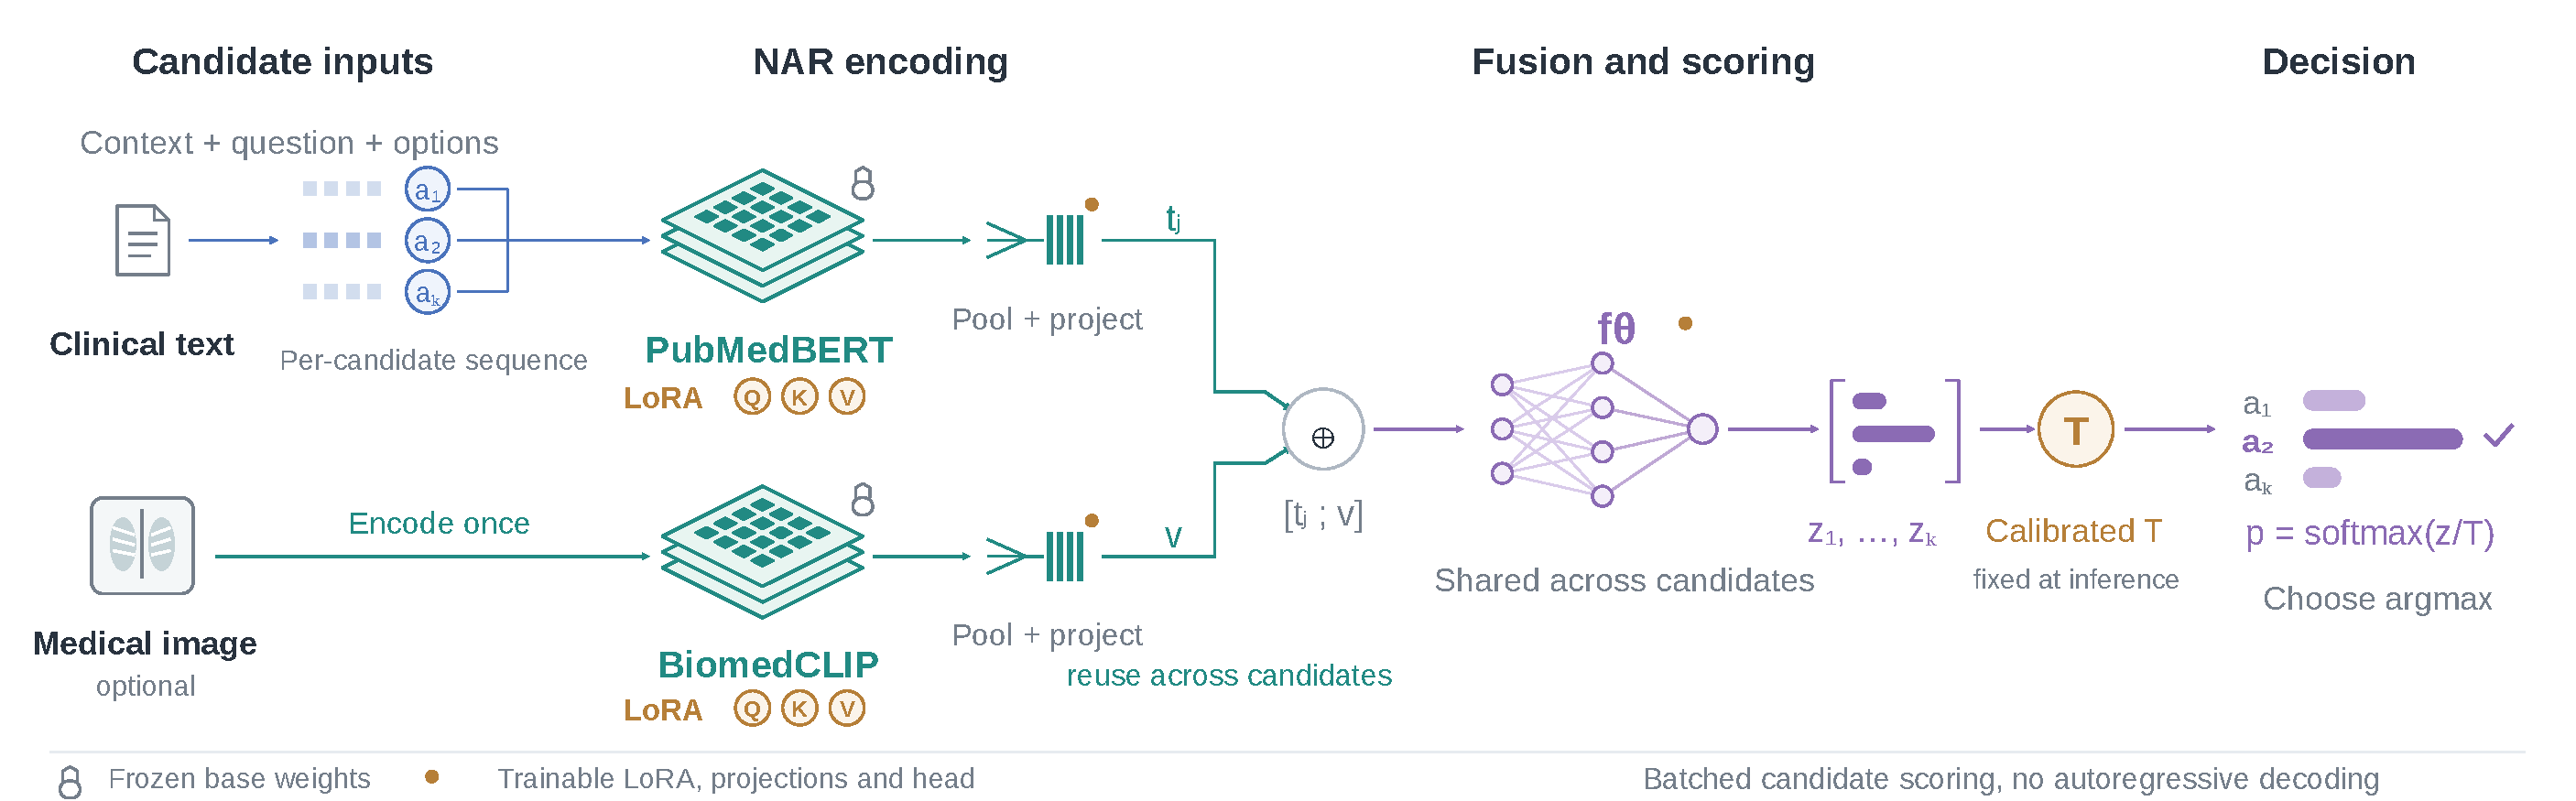
\includegraphics[width=\linewidth]{assets/figures/layamed_multimodal_nar.pdf}
\caption{\textbf{Laya-Med architecture supplied with the study.} PubMedBERT text representations and a BiomedCLIP image representation feed projections, fusion, and a shared candidate scorer. A fitted positive temperature changes probabilities but preserves the argmax. The absent-image representation and all training settings must be recorded with the checkpoint.}
\label{fig:layamed}
\end{figure}

\section{Post-hoc Result Reconciliation}
\label{app:audit}

Table~\ref{tab:reportedpolicies} preserves the draft's policy values without treating the apparent differences as paired gains. The source calls threshold rejection ``routing'' and labels one configuration MedGemma-Direct; we retain that model name and use ``threshold'' to describe the measured acceptance operation. The superscript in each policy cell is the number rejected out of 50. Base rows are copied as printed, but their denominators are not specified in the source.

Several issues require the original result records. First, the base rows differ from the main landscape table. Second, some zero-abstention conformal rows change accuracy, which is incompatible with an unchanged predictor and the singleton margin rule described in Section~\ref{sec:policies} when evaluated on identical examples. Third, one-decimal percentages must be checked against integer accepted counts; for example, 98.0\% on 48 accepted examples is not the one-decimal accuracy of an integer number of correct answers. These checks identify ambiguity, not its cause.

A further issue is aggregation. If a model abstains on every example in a dataset, accepted accuracy for that dataset is undefined. Such a dataset must not silently disappear from a cross-method average, nor be assigned zero accuracy without a stated utility convention. Report the accepted counts and task coverage explicitly. Conformal set coverage should also be computed directly from set membership, rather than substituted with singleton accuracy or the percentage of examples accepted.

\begin{table}[p]
\centering\scriptsize\setlength{\tabcolsep}{4pt}\renewcommand{\arraystretch}{1.22}
\caption{\textbf{Reported post-hoc results: unreconciled source values.} Each policy cell reports accepted accuracy and the rejected count $^{a/50}$. Base rows and method names are retained as printed. A dash with $^{50/50}$ means that no answers were accepted; a plain dash means unsupported. The source averages are omitted because their task support and pairing are not established. These values are not used as evidence of a fixed-model gain.}
\label{tab:reportedpolicies}
\begin{tabular*}{\linewidth}{@{\extracolsep{\fill}}lrrrrrrr@{}}
\toprule
\textbf{Method / policy} & PubMedQA & MedQA & MedMCQA & VQA-RAD & SLAKE & PathVQA & PMC-VQA\\
\midrule
\textbf{MedGemma-LL} & 71.4 & 49.2 & 60.2 & 70.6 & 79.4 & 62.3 & 48.7\\
\quad Threshold & $66.0^{3/50}$ & $48.0^{4/50}$ & $66.0^{1/50}$ & $78.0^{0/50}$ & $74.0^{0/50}$ & $70.0^{2/50}$ & $48.0^{2/50}$\\
\quad Conformal & $67.4^{4/50}$ & $55.3^{12/50}$ & $68.1^{3/50}$ & $81.3^{2/50}$ & $78.7^{3/50}$ & $72.1^{7/50}$ & $52.2^{4/50}$\\
\addlinespace[4pt]
\textbf{MedJev} & 63.8 & 28.3 & 35.9 & -- & -- & -- & --\\
\quad Threshold & $56.0^{37/50}$ & $24.0^{41/50}$ & $38.0^{47/50}$ & -- & -- & -- & --\\
\quad Conformal & $75.0^{26/50}$ & $12.5^{34/50}$ & $42.9^{36/50}$ & -- & -- & -- & --\\
\addlinespace[4pt]
\textbf{Laya} & 56.6 & 21.1 & 27.7 & -- & -- & -- & --\\
\quad Threshold & $56.0^{28/50}$ & $0.0^{49/50}$ & $0.0^{45/50}$ & -- & -- & -- & --\\
\quad Conformal & $57.5^{10/50}$ & $33.3^{38/50}$ & $6.7^{35/50}$ & -- & -- & -- & --\\
\addlinespace[4pt]
\textbf{MedGemma-Head} & 65.6 & 51.5 & 65.5 & 76.1 & 86.8 & 86.3 & 57.1\\
\quad Threshold & $62.0^{25/50}$ & $52.0^{41/50}$ & $70.0^{32/50}$ & $82.0^{22/50}$ & $88.0^{3/50}$ & $96.0^{4/50}$ & $52.0^{36/50}$\\
\quad Conformal & $62.2^{5/50}$ & $59.0^{11/50}$ & $74.4^{7/50}$ & $84.8^{4/50}$ & $88.0^{0/50}$ & $96.0^{0/50}$ & $53.7^{9/50}$\\
\addlinespace[4pt]
\textbf{MedGemma-Direct} & 72.6 & 53.3 & 68.7 & 69.7 & 90.7 & 90.0 & 57.2\\
\quad Threshold & $73.5^{1/50}$ & $74.1^{23/50}$ & $77.1^{15/50}$ & $83.7^{1/50}$ & $84.0^{0/50}$ & $95.8^{2/50}$ & $72.7^{17/50}$\\
\quad Conformal & $90.0^{0/50}$ & $44.0^{0/50}$ & $50.0^{0/50}$ & $100.0^{0/50}$ & $100.0^{0/50}$ & $100.0^{0/50}$ & $52.0^{0/50}$\\
\addlinespace[4pt]
\textbf{Laya-Med} & 64.0 & 30.4 & 40.8 & 56.0 & 80.0 & 86.9 & 45.4\\
\quad Threshold & $71.8^{11/50}$ & $--^{50/50}$ & $--^{50/50}$ & $55.3^{12/50}$ & $90.7^{7/50}$ & $94.4^{14/50}$ & $--^{50/50}$\\
\quad Conformal & $90.0^{0/50}$ & $38.9^{32/50}$ & $50.0^{40/50}$ & $98.0^{2/50}$ & $100.0^{1/50}$ & $100.0^{0/50}$ & $56.4^{11/50}$\\
\addlinespace[4pt]
\bottomrule
\end{tabular*}
\end{table}


The required reconciliation is one paired export per model and checkpoint. Recompute full-coverage accuracy, prediction-set coverage, singleton rate, and selective accuracy from that export; then compare threshold and conformal policies at matched retained coverage. If actual escalation is evaluated, include fallback errors and total latency. Until these records are available, the paper's post-hoc section specifies and audits the evaluation but does not establish an empirical reliability improvement.
